\documentclass{article}

\usepackage{longtable}
\usepackage{footnote}

\usepackage{indentfirst}
\usepackage{tabto}

\usepackage[utf8]{inputenc}
\usepackage[T1]{fontenc}
\usepackage{fancyhdr}
\usepackage{geometry}
\usepackage{array}
\usepackage[usenames,dvipsnames,svgnames,table]{xcolor}
\usepackage{multirow}
\usepackage{morefloats}
\usepackage{float}
\usepackage{soul}
\usepackage{color}
\usepackage{seqsplit}
\usepackage{gensymb}
\usepackage{siunitx}
\usepackage{graphicx}
\usepackage{pdfpages}
\usepackage[framemethod=TikZ]{mdframed}
\setcounter{secnumdepth}{3}

\usepackage[procnames]{listings}
\usepackage{color}

\definecolor{keywords}{RGB}{255,0,90}
\definecolor{comments}{RGB}{0,0,113}
\definecolor{red}{RGB}{160,0,0}
\definecolor{green}{RGB}{0,150,0}

\lstset{language=Python,
        basicstyle=\ttfamily\small,
        keywordstyle=\color{keywords},
        commentstyle=\color{comments},
        stringstyle=\color{red},
        % showstringspaces=false,
        identifierstyle=\color{green},
        procnamekeys={def,class}}


\restylefloat{table}

\fontfamily{cmss}\selectfont

\geometry{top = 1in, bottom = 1in, left = 0.5in, right = 0.5in}

\setlength{\parindent}{4em}
\setlength{\parskip}{1em}
\renewcommand{\baselinestretch}{1.5}

\pagestyle{fancy}
\renewcommand{\footrulewidth}{1pt}
\lhead{Waggle Sensor Array}
\chead{Interface and Data Format Specification}
\rhead{Version 1.0}
\lfoot{Waggle Group}
\rfoot{info@wa8.gl, park708@purdue.edu}

\setlength{\tabcolsep}{10pt}
\renewcommand{\arraystretch}{1.0}

%%%%%%%%%%%%%%%%%%%%%%%%%%%%%%%%%%%%%%%%%%%%%%%%%%%%%%%%%%%%%%%%%%%%%%%%%%%%

\begin{document}

\begin{titlepage}
   \vspace*{\stretch{1.0}}
   \begin{center}
        \Huge\textbf{\textsc{Interface and \\ Data Format Specification \\ for sensors \\
        \Large\textsc(v3 sensor boards with Alpha sensor, \\ Firmware version 4.1)}}\\[0.5cm]
        \Large\textsc{Waggle Group \\ Waggle Sensor Array}\\[1cm]
        \large\textsc{November 2017, }
        \large\textsc{Version 1.0}\\
   \end{center}
   \vspace*{\stretch{2.5}}
\end{titlepage}

\tableofcontents
\newpage

\section{Physical Connections and Interfaces}

\begin{figure}[h]
\begin{center}
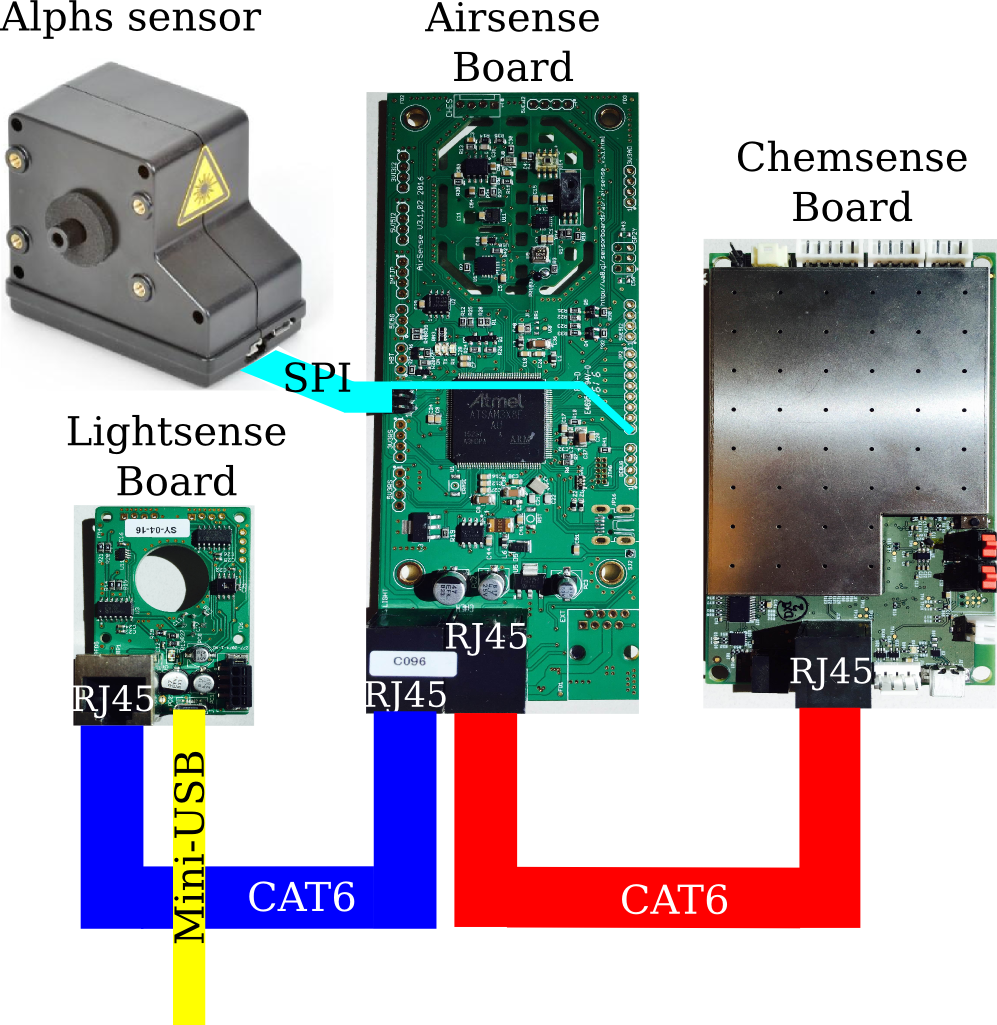
\includegraphics[width=4in]{physicalConnections.png}
\caption{Connections between the sensor boards and the sensor}
\label{fig:a}
\end{center}
\end{figure}


`v3 sensor boards with alpha sensor' means a set of sensors that are implemented on a v3.1 Metsense board, a v3.1 Lightsense board, and a Chemsense board and an independent alpha sensor.
\par
Physical connections between sensor boards and an alpha sensor are shown in the Figure \ref{fig:a}. A lightsense board and a chemsense board are connected to a metsense board through CAT6 cable. The metsense and the lightsense deliver data through I2C communication, and the chemsense board delivers data through serial3 communication. Alpha sensor is conncted to the metsense on SPI pins and one of GPIT pins. User requests and collects data from alpha sensor using SPI communication. All sensor data from metsense board, lightsense board, chemsense board, and alpha sensor are delivered to nodecontroller thourgh USB line attached on lightsense board using Serial communication. 

\newpage
\section{Data Transmission} \label{section:overall}

The data from the sensor boards are packetized in a transmission pacekt with the form of as they had read from the sensor. A transmission packet can be composed of several data sub-packets, each of which carries information pertaining to the parameter.
The transmission packet format and the data sub-packets are described here.

\subsection{Transmission Packet}
A transmission packet can be separated into 6 segments.
The structure of the transmission packet relies on positions of Bytes and predefined values for those Byte segments. 
Table 1 below illustrates how the segments are organized in a transmission packet.
\\

\begin{table}[h!]
\begin{minipage}{\textwidth}
    \centering
    \caption{Transmission Packet structure}
    \label{table:tran}
    \begin{tabular}{|c|c|c|c|c|c|c|}
        \hline
        \rowcolor{black!8}
        \textbf{Preamble} & \textbf{a~\footnote{Packet Type | Protocol Version}} & \textbf{Data Length} & \textbf{b~\footnote{Last Packet Flag | Sequence}} & \textbf{Data} & \textbf{CRC} & \textbf{Postscript}\\
        \hline
        \multirow{2}{*}{1st Byte} & \multirow{2}{*}{2nd Byte} & \multirow{2}{*}{3rd Byte} & \multirow{2}{*}{4th Byte} & next Bytes & \multirow{2}{*}{Penultimate Byte} & \multirow{2}{*}{Final Byte} \\ 
        & & & & up to 255 Bytes & & \\ \hline
    \end{tabular}
\end{minipage}
\end{table}

A description how the segments are organized in a transmission packet is shown in table 2 below.

\begin{table}[H]
    \centering
    {
    \begin{tabular}{|c|c|c|c|}
        \hline
        \rowcolor{black!8}
        \textbf{Field} & \textbf{Value} & \textbf{Segment} & \textbf{Length}\\
        \hline
        Preamble & 0xAA & 1 & 1 Byte\\ \hline
        \multirow{3}{*}{Packet Type} & 0x00: request & \multirow{4}{*}{2} & \multirow{3}{*}{1 Nibble} \\
         & 0x01: sensor reading & & \\ 
         & 0x02: bus reading & & \\ \cline{1-2} \cline{4-4}
        Protocol version & 0x02 &  & 1 Nibble\\ \hline
        Length of data & Variable & 3 & 1 Byte\\ \hline
        \multirow{2}{*}{Last Packet flag} & 0x01: last packet for one request & \multirow{3}{*}{4} & \multirow{2}{*}{1 bit} \\
         & 0x00: not last packet & & \\ \cline{1-2} \cline{4-4}
        Packet sequence & Variable &  & 7 bits \\ \hline
        Data & Variable & 5 & Variable \\ \hline
        CRC of data & Variable & 6 & 1 Byte\\ \hline
        Postscript & 0x55 & 7 & 1 Byte\\ \hline
    \end{tabular}
    }
    \caption{Transmission Packet Segments}
    \label{table:seg}
\end{table}


The first segment is the start byte, or the preamble. The preamble is followed by the packet type and protocol version, each of which are 4 bits long and are together packed into a single byte. Packet type is differed with regard to the purpose of the packet. When the packet sent from plugin to firmware, the type is ``requres'', and when the packet sent from firmware, type of the packet could be ``sensor reading'' or ``bus reading''. Type ``sensor reading'' means the data packetized in the packet are readings from sensors, which are sorted with sensor id given by Waggle group, and ``bus reading'' means the data packetized in the packet are readings from sensors that do not have given sensor id but connected on metsense board so that firmware can collect data from.
Next, one byte field that reports the first 1 bit of last packet flag and 7 bit sequence number. Following byte reports length of the data which comes along until its
immediately. The data segment is followed by a single CRC byte, and finally the packet ends with a one byte
crc and postscript. Table \ref{table:seg} lists the packet and the static values, if any, for each of the segments.
\\


\subsection{Data Sub-packets} \label{ssec:sub-pack}

The data segment of the transmission packet can be further separated into many sub-packets.
Two types of sub-packets are implemented, each of sub-packets are for sending request from coresense plugin to coresense firmware and visa versa.

Table \ref{table:toFW} below shows the organization of a sub-packet requesting sensor data.
The sub-pacekt starts with 4-bits call function id and 4-bits parameter length including source identifier, which is sensor id. The next bytes are parameters starting with target sensor id. Additional parameters can be attached after the sensor id. For more detail, refer sensor description file (SDF).

Table \ref{table:toPlugin} below shows the organization of a sub-packet sending sensor reading.
The sub-packet starts with a source identifier, which is sensor id. One bit validity field and seven bits ``length of the sub-packet'' field are packed together as the next byte. The length field counts the number of bytes following it which make up the sub-packet. 
The validity bit is set to 1 if the sensor reading is valid and set to 0 if the sensor is dead, disabled, unconnected, unresponsive or if data could not be collected
from the sensor in the time window. The size of the sub-packet is restricted to 127 Bytes by the seven bits length field.
\\



\begin{table}[H]
\begin{minipage}{\textwidth}
    \centering
    {
    \begin{tabular}{|c|c|c|}
        \hline
        \rowcolor{black!8}
        \textbf{Call Function ID} & \textbf{1-bit Acknowledge | Parameter Length} & \textbf{Parameters~\footnote{For sensors have sensor id, 1st Byte is SENSOR ID; For sensors collect data through bus functions, 1st Byte is bus type and 2nd Byte is BUS ADDRESS}} \\ \hline
        1 byte & 1 Byte & up to 252 Bytes \\
        \hline
    \end{tabular}
    }
    \caption{Transmission Packet Segments from plugin to firmware}
    \label{table:toFW}
\end{minipage}
\end{table}


\begin{table}[H]
\begin{minipage}{\textwidth}
    \centering
    {
    \begin{tabular}{|c|c|c|}
        \hline
        \rowcolor{black!8}
        \textbf{Source ID} & \textbf{1-bit Validity [0: invalid, 1: valid] | 7-bits Data Length} & \textbf{Data~\footnote{For sensors have sensor id, 1st Byte is SENSOR ID; For sensors collect data through bus functions, 1st Byte is bus type and 2nd Byte is BUS ADDRESS}} \\ \hline
        1 Byte & 1 Byte & up to 127 Bytes \\
        \hline
    \end{tabular}
    }
    \caption{Transmission Packet Segments}
    \label{table:toPlugin}
\end{minipage}
\end{table}



\subsection{Data Packer CRC} \label{ssec:crc-calc}

To validate the data transmitted from and to the sensor board, a CRC value for the data is
calculated and transmitted as part of the data packet. The Maxim 1-Wire
CRC polynomial is used for calculating the CRC.  On receiving the packet, the CRC is recalculated and compared with the value transmitted as part of
the packet. If the two CRC values match, the transmission is error-free.
The equivalent polynomial function of the CRC is shown in Equation \ref{eq:CRC}.

\begin{equation}
\label{eq:CRC}
CRC = x^8 + x^5 + x^4 + 1
\end{equation}

Further description of the Maxim 1-Wire CRC is available in Maxim Application Note 27. Below are
the Python and C implementations of the CRC calculator. The CRC implementations below take a
data Byte and the previous CRC as inputs, and return the new CRC as return value.
\\

\textbf{Python Code:}
\begin{mdframed}
\begin{lstlisting}
def calc_crc (data_Byte,CRC_Value)
    CRC_Value = ord(data_Byte) ^ CRC_Value
    for j in range(8):
    if (CRC_Value  & 0x01):
        CRC_Value  = (CRC_Value  >> 0x01) ^ 0x8C
    else:
        CRC_Value  =  CRC_Value  >> 0x01
return CRC_Value
\end{lstlisting}
\end{mdframed}

\vskip 0.1in
\textbf{C Code:}
\begin{mdframed}
\begin{lstlisting}
unsigned char  CRC_CALC (unsigned char data, unsigned char crc) 
{ 
        unsigned char i;
        crc ^= data;
        for (i=0x00; i < 0x08; i++)
        {
                if (crc & 0x01) { crc = (crc >> 0x01)^0x8C; }
                else { crc =  crc >> 0x01; }
        }
        return(crc);
}
\end{lstlisting}
\end{mdframed}
\newpage
\section{Sub-packets from Coresense}

As shortly explained in document section \ref{ssec:sub-pack}, data sub-packets from metsense board, lightsense board, chemsense board, and alpha sensor are generated depending on its data reading from each sensor if valid. The first byte of the sub-packets from those sensor boards/sensor is sensor ID, and the first bit of second byte means validity of the packet and next 7 bits of the second byte is length of the sensor data. Data length and type of sensor reading are shown in Table \ref{table:dataChunk}. Detail of sub-packet and sensor data will be explined following sections.


\subsection{Parameters}

The sensor boards output a set of parameters which are identified by a unique ID. Each parameter
has a set of values associated with it which are encoded in an appropriate data format. The table
below lists the various parameters produced by the sensor boards, the unique source ID used to identify them, the values produced by them.


\begin{center}
\begin{longtable}{|l|c|>{\centering}p{0.3\textwidth}|c|}
\caption{Data sub-packet structure (each row is a ``chunk'')} \label{table:dataChunk} \\

\hline \rowcolor{black!8} \multicolumn{1}{|c|}{\textbf{Parameter}} & \multicolumn{1}{c|}{\textbf{Source ID}} & \multicolumn{1}{c|}{\textbf{Values}} & \multicolumn{1}{c|}{\textbf{Data Length}} \\ \hline
\endfirsthead

\multicolumn{4}{c}%
{{\bfseries \tablename \thetable{} -- continued from previous page}} \\
\hline \rowcolor{black!8} \multicolumn{1}{|c|}{\textbf{Parameter}} & \multicolumn{1}{c|}{\textbf{Source ID}} & \multicolumn{1}{c|}{\textbf{Values}} & \multicolumn{1}{c|}{\textbf{Data Length}} \\ \hline 
\endhead

\rowcolor{black!8} \multicolumn{4}{|r|}{{Continued on next page}} \\ \hline
\endfoot

\hline
\endlastfoot

        \multirow{3}{*}{Firmware version} & \multirow{3}{*}{0xFF} & Version (HW/SW) & 2 bytes \\ \cline{3-4}
        & & Build time & 4 bytes \\ \cline{3-4}
        & & Build git & 2 bytes \\ \hline

    \rowcolor{black!5} \multicolumn{4}{|c|}{{Metsense board}} \\ \hline
        Metsense/Lightsense MAC address & 0x00 & MAC Address & 6 bytes \\ \hline
        TMP112 & 0x01 & Temperature & 2 bytes \\ \hline
        \multirow{2}{*}{HTU21D} & \multirow{2}{*}{0x02} & Temperature & 2 bytes \\ \cline{3-4}
        & & Relative humidity & 2 bytes \\ \hline
        HIH4030 & 0x03 & Relative humidity & 2 bytes \\ \hline
        \multirow{2}{*}{BMP180} & \multirow{2}{*}{0x04} & Temperature & 2 bytes \\ \cline{3-4}
        & & Pressure & 3 bytes  \\ \hline
        PR103J2 & 0x05 & Temperature & 2 bytes \\ \hline
        TSL250RD & 0x06 & Visible Light & 2 bytes \\ \hline
        \multirow{4}{*}{MMA8452Q} & \multirow{4}{*}{0x07} & Acceleration in X & 2 bytes \\ \cline{3-4}
        & & Acceleration in Y & 2 bytes \\ \cline{3-4}
        & & Acceleration in Z & 2 bytes \\ \hline
        SPV1840LR5H-B & 0x08 & RMS Sound Level & 128 bytes \\ \hline
        TSYS01 & 0x09 & Temperature & 2 bytes \\ \hline
        
    \rowcolor{black!8} \multicolumn{4}{|c|}{{Lightsense board}} \\ \hline
        \multirow{3}{*}{HMC5883L} & \multirow{3}{*}{0x0A} & Magnetic Field in Z & 2 bytes \\ \cline{3-4}
        & & Magnetic Field in Y & 2 bytes \\ \cline{3-4}
        & & Magnetic Field in Z & 2 bytes \\ \hline
        \multirow{2}{*}{HIH6130} & \multirow{2}{*}{0x0B} & Temperature & 2 bytes \\ \cline{3-4}
        & & Relative humidity & 2 bytes \\ \hline
        APDS-9006-020 & 0x0C & Ambient light intensity & 3 bytes \\ \hline
        TSL260RD & 0x0D & IR intensity & 3 bytes \\ \hline
        TSL250RD & 0x0E & Visible light intensity & 3 bytes \\ \hline
        MLX75305 & 0x0F & Light & 3 bytes \\ \hline 
        ML8511 & 0x10 & UV intensity & 3 bytes \\ \hline
        TMP421 & 0x13 & Temperature & 2 bytes \\ \hline

    \rowcolor{black!8} \multicolumn{4}{|c|}{{Chemsense board}} \\ \hline
        Chemsense configuration & 0x16 & Chemsense FW config & 1514 bytes \\ \hline
        Chemsense reading & 0x2A & Raw reading & Varies \\ \hline

     \rowcolor{black!8} \multicolumn{4}{|c|}{{Alpha Sensor}} \\ \hline
        \multirow{9}{*}{Histogram} & \multirow{9}{*}{0x28} & Bin count & 32 bytes \\ \cline{3-4}
        & & Average time & 4 bytes \\ \cline{3-4}
        & & Sample flow rate & 4 bytes \\ \cline{3-4}
        & & Temp/Pressure(alter) & 4 bytes\\ \cline{3-4}
        & & Sampling period & 4 bytes \\ \cline{3-4}
        & & Sum of the counts & 2 bytes \\ \cline{3-4}
        & & PM 1 & 4 bytes \\ \cline{3-4}
        & & PM 2.5 & 4 bytes \\ \cline{3-4}
        & & PM 10 & 4 bytes \\ \hline
        Serial & 0x29 & Serial number & 20 bytes \\ \hline
        \multirow{4}{*}{Status} & \multirow{4}{*}{0x2B} & FanON & 1 byte \\ \cline{3-4}
        & & LaserON & 1 byte \\ \cline{3-4}
        & & FanDACVal & 1 byte \\ \cline{3-4}
        & & LaserDACVal & 1 byte \\ \hline
        Firmware & 0x30 & Firmware version & 2 bytes \\ \hline
        \multirow{10}{*}{Configuration} & \multirow{5}{*}{0x31} & Bin Boundaries & 32 bytes \\ \cline{3-4}
        & & Bin particle volumes & 64 bytes \\ \cline{3-4}
        & & Bin particle densities & 64 bytes \\ \cline{3-4}
        & & Bin sample volume weightings & 64 bytes \\ \cline{3-4}
        & & Gain scaling coefficient & 4 bytes \\ \cline{3-4}
        & & Sample flow rate & 4 bytes \\ \cline{3-4}
        & & Laser DAC & 1 byte \\ \cline{3-4}
        & & Fan DAC & 1 byte \\ \cline{3-4}
        & & Conversion factor & 1 byte \\ \cline{3-4}
        & & Spare bytes & 21 bytes \\ 

\end{longtable}
\end{center}


\newpage
\subsection{Data packets}
The context of each parameter, its utility and the arrangement of its values is described below. In all
the tables below, the validity bit is set to 1, which means the data is valid. The parameter described
below are aggregated based on the sensor-board they are situated on -
Metsense, Lightsense and Chemsense.

\subsubsection{Firmware Version}
This is a 8 bytes version information that identifies hardware version, software version, and build information of the waggle node.
The build time and the build git are included to varify the effectiveness of the software.
Firmware version is bit masked and encoded through format 1, and build git is encoded through format 1.

\begin{table}[h!]
    \centering
    \caption{Sub-packet of Firmware version}
    \begin{tabular}{|c|c|c|c|c|}
        \hline
        \rowcolor{black!8}
        \textbf{0xFD} & \textbf{0x88} & \textbf{Firmware version} & \textbf{Build time} & \textbf{Build git} \\ \hline
        Byte[0] & Byte[1] & Bytes[2 -- 3] & Bytes[4 -- 7] & Bytes[8 -- 9]\\ \hline
    \end{tabular}
\end{table}


\newcolumntype{a}{>{\columncolor{black!8}}c}
\begin{table}[h!]
    \centering
    \caption{Firmware version}
    \begin{tabular}{|a|c|}
        \hline
        \textbf{3 bit major HW ver. | 3 bit minor HW ver. | 2 bit major SW ver.} & Byte[2] \\ \hline
        \textbf{2 bit major SW ver. | minor SW ver. $\times$ 10 + sub SW ver.} & Byte[3]\\ \hline
    \end{tabular}
\end{table}


\subsubsection{Metsense}

\paragraph{$\bullet$ Metsense/Lightsense MAC address: }

This is a 6-byte ID that uniquely identifies each Airsense board. This MAC address is also applied to each Lightsense board which has the same board number. The ID is provided by a DS2401 1-Wire DSN chip. The 1-byte family ID and CRC provided by the DSN chip are omitted, and the rest 6 bytes are used as the Unique ID.


\begin{table}[h!]
    \centering
    \caption{Sub-packet of met/lightsense board MAC address}
    \begin{tabular}{|c|c|c|}
        \hline
        \rowcolor{black!8}
        \textbf{0x00} & \textbf{0x86} & \textbf{MAC address} \\
        \hline
        Byte[0] & Byte[1] & Bytes[2 -- 7]\\ \hline
    \end{tabular}
\end{table}
\par

\paragraph{$\bullet$ TMP112, HIH4030, PR103J2, TSL250RD, TSYS01:}

TMP112, PR103J2, and TSYS01 are temperature sensors, HIH4030 is a humidity sensor, and TSL250RD is a light sensor.
The coresense firmware collectes data from TMP112 through I2C, and from other sensors using analog read.
All the reading values from the sensors are packetized as the raw value as they are collected.
The raw reading will be converted relatively to temperature in centigrade, humidity in \%RH, and light in lux.

\begin{table}[h!]
    \centering
    \caption{Sub-packet for the sensor listed above}
    \begin{tabular}{|c|c|c|}
        \hline
        \rowcolor{black!8}
        \textbf{Sensor ID} (0x01, 0x03, 0x05, 0x06, 0x09) & \textbf{0x82} & \textbf{Raw sensor reading} \\
        \hline
        Byte[0] & Byte[1] & Bytes[2 -- 3]\\ \hline
    \end{tabular}
\end{table}


\paragraph{$\bullet$ HTU21D:}
HTU21D is a temperature and relative humidity sensor.
The coresense firmware collects data from HTU21D through I2C and the readings are packetized as the raw value as they are collected.
The raw readings will be converted to temperature in centigrate, humidity in \%RH.
\\

\begin{table}[h!]
    \centering
    \caption{Sub-packet of a temperature and relative humidity sensor, HTU21D}
    \begin{tabular}{|c|c|c|c|}
        \hline
        \rowcolor{black!8}
        \textbf{0x02} & \textbf{0x84} & \textbf{Raw temperature reading} & \textbf{Raw humidity reading}\\
        \hline
        Byte[0] & Byte[1] & Bytes[2 -- 3] & Bytes[4 -- 5] \\ \hline
    \end{tabular}
\end{table}


\paragraph{$\bullet$ BMP180:}

BMP180 is a temperature and barometric pressure sensor.
The coresense firmware collects data from BMP180 through I2C and the readings are packetized as the raw value as they are collected. 
The raw readings will be converted to temperature in centigrade and barometric pressure in hPa.
\\


\begin{table}[h!]
    \centering
    \caption{Sub-packet of a temperature and barometric pressure sensor, BMP180}
    \begin{tabular}{|c|c|c|c|}
        \hline
        \rowcolor{black!8}
        \textbf{0x04} & \textbf{0x84} & \textbf{Raw temperature reading} & \textbf{Raw pressure reading}\\
        \hline
        Byte[0] & Byte[1] & Bytes[2 -- 3] & Bytes[4 -- 5] \\ \hline
    \end{tabular}
\end{table}

\paragraph{$\bullet$ MMA8452Q:}

MMA8452Q is a three-axis accelerometer. The accelerations in three orthogonal directions, x, y and z, as a multiple of acceleration due to gravity (g) are obtained from the sensor. The coresense firmware collects data from this sensor through I2C and the readings are packetized as the raw value as they are collected.
The raw reading will be converted to a vibration value (represented as multiple of g) and three directional acceleration in g.

\begin{table}[h!]
    \centering
    \caption{Sub-packet of a three-axis accelerometer, MMA8452Q}
    \begin{tabular}{|c|c|c|c|c|}
        \hline
        \rowcolor{black!8}
        \textbf{0x07} & \textbf{0x86} & \textbf{Raw Ax reading} & \textbf{Raw Ay reading} & \textbf{Raw Az reading}\\
        \hline
        Byte[0] & Byte[1] & Bytes[2 -- 3] & Bytes[4 -- 5] & Bytes[6 -- 7] \\ \hline
    \end{tabular}
\end{table}

\paragraph{$\bullet$ SPV1840LR5H-B:}

SPV1840LR5H is a MEMS microphone that is sampled at high frequency to obtain the peaks and calculate the sound intensity for a time window.
The coresense firmware collects data from this sensor through analog read and the readings are packetized as the raw value as they are collected.
The raw readings will be converted to sound level in dB.
\\

\begin{table}[h!]
    \centering
    \caption{Sub-packet of a sound level sensor, SPV1840LR5H-B}
    \begin{tabular}{|c|c|c|}
        \hline
        \rowcolor{black!8}
        \textbf{0x08} & \textbf{0xFF} & \textbf{64 times of Raw reading} \\
        \hline
        Byte[0] & Byte[1] & Bytes[2 -- 129]\\ \hline
    \end{tabular}
\end{table}


\subsubsection{Lightsense}

\paragraph{$\bullet$ HMC5883L:}
HMC5883L is a three-axis magnetometer. The magnetic field strengths in three orthogonal directions, x, y and z are obtained from the sensor.
The coresense firmware collects data from this sensor through I2C and the readings are packetized as the raw value as they are collected.
The raw readings will be converted to three directional magnetic field in G.
\\

\begin{table}[h!]
    \centering
    \caption{Sub-packet of a three-axis magnetometer, HMC5883L}
    \begin{tabular}{|c|c|c|c|c|}
        \hline
        \rowcolor{black!8}
        \textbf{0x0A} & \textbf{0x86} & \textbf{Raw Hx reading} & \textbf{Raw Hy reading} & \textbf{Raw Hz reading}\\
        \hline
        Byte[0] & Byte[1] & Bytes[2 -- 3] & Bytes[4 -- 5] & Bytes[6 -- 7] \\ \hline
    \end{tabular}
\end{table}



\paragraph{$\bullet$ HIH6130:}
HIH6130 is a temperature and relative humidity sensor.
The coresense firmware collects data from HIH6130 through I2C and the readings are packetized as the raw value as they are collected.
The raw readings will be converted to temperature in centigrate, humidity in \%RH.
\\

\begin{table}[h!]
    \centering
    \caption{Sub-packet of a temperature and relative humidity sensor, HIH6130}
    \begin{tabular}{|c|c|c|c|}
        \hline
        \rowcolor{black!8}
        \textbf{0x0B} & \textbf{0x84} & \textbf{Relative Humidity in Format 6} & \textbf{Temperature in Format 6} \\
        \hline
        Byte[0] & Byte[1] & Bytes[2 -- 3] & Bytes[4 -- 5] \\ \hline
    \end{tabular}
\end{table}


\paragraph{$\bullet$ APDS-9006-020, TSL260, TSL250, MLX75305, and ML8511:}
APDS-9006-020, TSL260, TSL250, MLX75305, and ML8511 are light sensors that produce the analog voltage 
representing in general luminance, irradiance measured in $\mu$W/cm$^2$, or UV index. 
The coresense firmware collects data from sensors listing above through I2C and the reading is packetized as the raw value as it is collected.
The raw reading will be converted to temperature in centigrate, humidity in \%RH.

\begin{table}[h!]
    \centering
    \caption{Sub-packet of light intensity sensors, APDS-9006-020, TSL260, TSL250, MLX75305, and ML8511}
    \begin{tabular}{|c|c|c|c|}
        \hline
        \rowcolor{black!8}
        \textbf{Sensor ID} (0x0C $\sim$ 0x10) & \textbf{0x82} & \textbf{Voltage output in Format 1}\\
        \hline
        Byte[0] & Byte[1] & Bytes[2 -- 3] \\ \hline
    \end{tabular}
\end{table}


\paragraph{$\bullet$ TMP421:}
TMP421 is a temperature sensor.
The coresense firmware collects data from TMP421 through I2C and the reading is packetized as the raw value as it is collected.
The raw reading will be converted to temperature in centigrate.

\begin{table}[h!]
    \centering
    \caption{Sub-packet of a temperature sensor, TMP421}
    \begin{tabular}{|c|c|c|}
        \hline
        \rowcolor{black!8}
        \textbf{0x13} & \textbf{0x82} & \textbf{Temperature in Format 6}\\
        \hline
        Byte[0] & Byte[1] & Bytes[2 -- 3] \\ \hline
    \end{tabular}
\end{table}


\subsubsection{Chemsense:}

Chemsense board sends data through Serial3 communication line in metsense board.
All sensor values from chemsense board are caluated in its own firmware.
The raw serial readings from the board are packetized as the raw value as they are collected, and the reading will be sorted out in database.

\paragraph{$\bullet$ Chemsense reading:}
To fully collect all the data from chemsense board, the firmware collect data three times in a row, so that coresense firmware sends three packets when it gets request of reading of chemsense board.

\begin{table}[h!]
    \centering
    \caption{Sub-packet of a chemsense board}
    \begin{tabular}{|c|c|c|}
        \hline
        \rowcolor{black!8}
        \textbf{0x2A} & \textbf{Varies} & \textbf{Raw reading}\\
        \hline
        Byte[0] & Byte[1] & Bytes[Vareis] \\ \hline
    \end{tabular}
\end{table}


\paragraph{$\bullet$ Chemsense firmware configuration:}
\textbf{THIS DATA DO NOT FOLLOW CORESENSE PACKET FORMAT, NO FORMAT AT ALL}
Chemsense Fiwmware configuration is one-time collectable charactor data, when the board is powered on.
The coresense firmware collectes data when the board is powered on, and store the data into an array.
The user can call this data with their own plugin (request and answer collecting functions).


\newcolumntype{a}{>{\columncolor{black!8}}c}
\begin{table}[h!]
    \centering
    \caption{Sub-packet of chemsense firmware configuration}
    \begin{tabular}{|a|c|}
        \hline
        \textbf{1st line} & ``Start sending Chemsense FW configuration'' \\ \hline
        \textbf{2nd -- 48th line} & Each raw reading line (Character) \\ \hline
        \textbf{last line} & ``End sending Chemsense FW configuration'' \\ \hline
    \end{tabular}
\end{table}


\subsubsection{Alpha Sensor:}
Coresense firmware communicates with alpha sensor through SPI.
The raw SPI readings from the board are packetized as the raw value as they are collected, and the reading will be sorted out in database.
In this document, concise Alpha sensor information is provided. For more information, refer to \textbf{`Firmware commands version 18.xls' and `OPC-N2 Manual Issue December 2015.pdf'} at \textbf{`waggle/docs/alphasense-opc-n2'}.

\paragraph{$\bullet$ Histogram}
Histogram of alpha sensor is 62 bytes of reading. This parameter provides various information as listed below. \textbf{All data from the alpha sensor is LSB first}.

\begin{table}[h!]
    \centering
    \caption{Sub-packet Alpha sensor histogram}
    \begin{tabular}{|c|c|c|}
        \hline
        \rowcolor{black!8}
        \textbf{0x28} & \textbf{0xBE} & \textbf{Various sensor information as listed above}\\
        \hline
        Byte[0] & Byte[1] & Bytes[2 -- 63] \\ \hline
    \end{tabular}
\end{table}


\begin{itemize}
\setlength\itemsep{0em}
\item[$\circ$] Bin Counts (Bin0 - Bin15) are unsinged 16 bit integer variables (Bytes[2 -- 33]).
\item[$\circ$] An unsigned 8-bit integer represents the average amount of time that particles sized in the stated bin took cross the laser beam of the sensor. Value 10 represents 3.33 $\mu$s (Bytes[34 -- 37]).
\item[$\circ$] The sample flow rate in ml/s is provided as a float variable (Bytes[38 -- 41]).
\item[$\circ$] Temperature and Pressure alternating. Temperature is an unsigned 32-bit integer that represents temperature in Celsious multiplied by 10. Pressure is an unsigned 32-bit integer that represents pressure in pascals (Bytes[42 -- 45]).
\item[$\circ$] Actual sampling period of a measure of the historgam in seconds provided as 4 bytes of float variables (Bytes[46 -- 49]).
\item[$\circ$] The least significat 16-bit of the sum of the counts in all the histogram bins is provided by unsigned 16bit integers (Bytes[50 -- 51]).
\item[$\circ$] A float variable occupying 4 bytes for PM1. Unit is $\mu$g/m$^3$ (Bytes[52 -- 55]).
\item[$\circ$] A float variable occupying 4 bytes for PM2.5. Unit is $\mu$g/m$^3$ (Bytes[56 -- 59]).
\item[$\circ$] A float variable occupying 4 bytes for PM10. Unit is $\mu$g/m$^3$ (Bytes[60 -- 63]).
\end{itemize}


\begin{table}[h!]
    \centering
    \caption{Detail sub-packet of Alpha sensor histogram}
    \begin{tabular}{|>{\centering\arraybackslash}p{0.3\textwidth}|>{\centering\arraybackslash}p{0.2\textwidth}|}
        \hline
        \rowcolor{black!8}
        \textbf{Parameter} & \textbf{Data location}\\ \hline
        Bin Count (32 Bytes) & Bytes[2 - 33] \\ \hline
        Average Time (4 Bytes) & Bytes[34 -- 37] \\ \hline
        Sample flow rate (4 Bytes) & Bytes[38 -- 41] \\ \hline
        Temp/Pressure(alter) (4 Bytes) & Bytes[42 -- 45] \\ \hline
        Sampling period (4 Bytes) & Bytes[46 -- 49] \\ \hline
        Sum of the counts (2 Bytes) & Bytes[50 -- 51] \\ \hline
        PM1 (4 Bytes) & Bytes[51 -- 55] \\ \hline
        PM2.5 (4 Bytes) & Bytes[56 -- 59] \\ \hline
        PM10 (4 Bytes) & Bytes[60 -- 63] \\ \hline
    \end{tabular}
\end{table}



\paragraph{$\bullet$ Serial}
Serial of alpha sensor is 20 bytes of reading. This parameter provides the serial number of the alpha sensor by character.\\


\begin{table}[h!]
    \centering
    \caption{Sub-packet of Alpha sensor serial number}
    \begin{tabular}{|c|c|c|}
        \hline
        \rowcolor{black!8}
        \textbf{0x29} & \textbf{0x94} & \textbf{Raw values}\\
        \hline
        Byte[0] & Byte[1] & Bytes[2 -- 21] \\ \hline
    \end{tabular}
\end{table}


\paragraph{$\bullet$ Firmware}
Firmware of alpha sensor is 2 bytes of reading. This parameter provides the Firmware version of the alpha sensor by two unsigned 8-bit integer.\\


\begin{table}[h!]
    \centering
    \caption{Sub-packet of Alpha sensor firmware}
    \begin{tabular}{|c|c|c|}
        \hline
        \rowcolor{black!8}
        \textbf{0x30} & \textbf{0x82} & \textbf{Raw values}\\
        \hline
        Byte[0] & Byte[1] & Bytes[2 -- 3] \\ \hline
    \end{tabular}
\end{table}

\paragraph{$\bullet$ Status}
Status of alpha sensor is 4 bytes of reading. This parameter provides status of the alpha sensor in terms of if fan and laser are on/off and DAC value of the fan and laser.\\

\begin{table}[h!]
    \centering
    \caption{Sub-packet of Alpha sensor firmware}
    \begin{tabular}{|c|c|c|}
        \hline
        \rowcolor{black!8}
        \textbf{0x2B} & \textbf{0x84} & \textbf{Raw values}\\
        \hline
        Byte[0] & Byte[1] & Bytes[2 -- 5] \\ \hline
    \end{tabular}
\end{table}


\begin{table}[h!]
    \centering
    \caption{Detail sub-packet of Alpha sensor histogram}
    \begin{tabular}{|>{\centering\arraybackslash}p{0.3\textwidth}|>{\centering\arraybackslash}p{0.2\textwidth}|}
        \hline
        \rowcolor{black!8}
        \textbf{Parameter} & \textbf{Data location}\\ \hline
        Fan on/off (1 Byte, 0 or 1) & Bytes[2] \\ \hline
        Laser on/off (1 Byte, 0 or 1) & Bytes[3] \\ \hline
        Fan DAC value (1 Byte) & Bytes[4] \\ \hline
        Laser DAC value (1 Byte) & Bytes[5] \\ \hline
    \end{tabular}
\end{table}


\paragraph{$\bullet$ Configuration}
\textbf{THIS DATA DO NOT FOLLOW CORESENSE PACKET FORMAT, NO FORMAT AT ALL}
Configuration of alpha sensor is 256 bytes of reading. 
This parameter provides various information as listed below.
Since this configuration data is too long to fit into a sub-packet, the data are not packed into coresense packet.


\newcolumntype{a}{>{\columncolor{black!8}}c}
\begin{table}[h!]
    \centering
    \caption{Sub-packet of alpha sensor configuration}
    \begin{tabular}{|a|c|}
        \hline
        \textbf{1st line} & ``Start sending alpha sensor configuration'' \\ \hline
        \textbf{2nd line} & 256 bytes of raw reading (Binary) \\ \hline
        \textbf{last line} & ``End sending alpha sensor configuration'' \\ \hline
    \end{tabular}
\end{table}


\begin{itemize}
\setlength\itemsep{0em}
\item[$\circ$] Bin Boundaries (BB0 - BB14) are unsinged 16 bit integer variables, and two spare bytes.
\item[$\circ$] Bin Particle Volumes (BPV0 - BPV15) are float variables occupyting 4 bytes each.
\item[$\circ$] Bin Particle Densities (BPD0 -- BPD15) are float variables occupying 4 bytes each.
\item[$\circ$] Bin Sample Volume Weightings (BSVW0 -- BSVW15) are float variables occupying 4 bytes each.
\item[$\circ$] Gain Scaling Coefficient (GSC) is float variable occupying 4 bytes.
\item[$\circ$] Sample flow rate is a float variable occupying 4 bytes.
\item[$\circ$] Laser DAC value is unsigned 8bit interger variable.
\item[$\circ$] Fan DAC value is unsigned 8bit integer variable.
\item[$\circ$] Time of Flight to Sample Flow Rate conversion factor is unsigned 8bit integer variable.
\item[$\circ$] 21 spare bytes follow Configuration variables.
\end{itemize}


\makeatletter
\setlength{\@fptop}{0pt}
\makeatother

\begin{table}[h!]
    \centering
    \caption{Detail second lind of Alpha sensor configuration}
    \begin{tabular}{|>{\centering\arraybackslash}p{0.5\textwidth}|>{\centering\arraybackslash}p{0.2\textwidth}|}
    % \begin{tabular}{|c|c|}
        \hline
        \rowcolor{black!8}
        \textbf{Parameter} & \textbf{Data location}\\ \hline
        Bin Boundaries (32 Bytes) & Bytes[0 -- 31] \\ \hline
        Bin Particle Volumes (64 Bytes) & Bytes[32 -- 95] \\ \hline
        Bin Particle Densities (64 Bytes) & Bytes[96 -- 159] \\ \hline
        Bin Sample Volume Weightings (64 Bytes) & Bytes[160 -- 223] \\ \hline
        Gain Scaling Coefficient (4 Bytes) & Bytes[224 -- 227] \\ \hline
        Sample Flow Rate (4 Bytes) & Bytes[228 -- 231] \\ \hline
        Laser DAC (1 Byte) & Byte[232] \\ \hline
        Fan DAC (1 Byte) & Byte[233] \\ \hline
        Conversion factor (1 Byte) & Byte[244] \\ \hline
        Spare Bytes (21 Bytes) & Bytes[245 -- 255] \\ \hline
    \end{tabular}
\end{table}

\clearpage
\newpage
\section{Sensor Data Units}\label{section:parameterUnits}
\subsection { Raw and Processed} 


The sensor boards output a set of raw readings which need to be calculated for proper units for each of data.
The table below lists the various units for each sensor values.
`Current Units' in the table means the unit after conversion through designated equations stored in database currently (Nov, 2017), and `Processed Units' means the unit which will be updated in the future.

\begin{center}
\begin{longtable}{|l|c|c|c|}
\caption{Sensor units}
\label{table:parameterUnits} \\

\hline \rowcolor{black!8} \multicolumn{1}{|l|}{\textbf{Sensor/Parameter}} & \multicolumn{1}{c|}{\textbf{Current Units}} & \multicolumn{1}{c|}{\textbf{Processed Units}} & \multicolumn{1}{c|}{\textbf{Comments}} \\ \hline
\endfirsthead

\multicolumn{4}{c}%
{{\bfseries \tablename\ \thetable{} -- continued from previous page}} \\

\hline \rowcolor{black!8} \multicolumn{1}{|l|}{\textbf{Sensor/Parameter}} & \multicolumn{1}{c|}{\textbf{Current Units}} & \multicolumn{1}{c|}{\textbf{Processed Units}} & \multicolumn{1}{c|}{\textbf{Comments}} \\ \hline
\endhead

\rowcolor{black!8} \multicolumn{4}{|r|}{{Continued on next page}} \\ \hline
\endfoot

\hline
\endlastfoot
 
    Firmware version & No Units & No Units & \\ \hline

  \rowcolor{black!5} \multicolumn{4}{|c|}{{Airsense board}} \\ \hline
    Met/Lightsense MAC & No Units & No Units & \\  \hline
    TMP112 & \degree C & \degree C & \\ \hline
    HTU21D & \degree C, \%RH & \degree C, \%RH & \\ \hline
    BMP180 & \degree C, Pa & \degree C, Pa & \\ \hline
    PR103J2 & \degree C & \degree C & \\ \hline
    TSL250RD & Raw reading* & $\mu$w/m$^2$ & \\  \hline
    MMA8452Q & g, g, g & g, g, g, g & \\ \hline
    SPV1840LR5H-B & Raw reading* & & \\ \hline
    TSYS01 & \degree C & \degree C & \\ \hline
    
  \rowcolor{black!5} \multicolumn{4}{|c|}{{Lightsense board}} \\ \hline
    HMC5883L & G, G, G & G, G, G & \\ \hline
    HIH6130 & \degree C, \%RH & \degree C, \%RH & \\ \hline
    APDS-9006-020 & Raw reading & lux & \\  \hline
    TSL260RD & Raw reading* & $\mu$w/m$^2$ & \\  \hline
    TSL250RD & Raw reading* & $\mu$w/m$^2$ & \\  \hline
    MLX75305 & Raw reading* & $\mu$w/m$^2$ & \\  \hline
    ML8511 & Raw reading* & UV index & \\  \hline
    TMP421 & \degree C & \degree C & \\ \hline

  \rowcolor{black!5} \multicolumn{4}{|c|}{{Chemsense board}} \\ \hline
    Chemsense configuration & No unit & No unit & Don't need conversions \\ \hline
    Chemsense reading & Raw reading* & See Table \ref{table:tran} & \\ \hline

 \rowcolor{black!5} \multicolumn{4}{|c|}{{Alpha sensor}} \\ \hline 
    Serial & No unit & No unit & \\ \hline
    Firmware & No unit & No unit & \\ \hline
 
 \rowcolor{black!2} \multicolumn{4}{|c|}{{Alpha sensor -- Status}} \\ \hline
    FanON & No unit & No unit & \\ \hline
    LaserON & No unit & No unit & \\ \hline
    FanDACVal & No unit & No unit & \\ \hline
    LaserDACVal & No unit & No unit & \\ \hline

 \rowcolor{black!2} \multicolumn{4}{|c|}{{Alpha sensor -- Histogram}} \\ \hline
    Bin count & No unit & No unit & \\ \hline
    Average time & Raw reading* & $\mu$s & value 10 = 3.33 $\mu$s \\ \hline
    Sample flow rate & Raw reading* & ml/s & \\ \hline
    Temp/Pressure(alter) & Raw reading* & $^{\circ}$C / hPa (alter) & \\ \hline
    Sampling period & Raw reading* & s & \\ \hline
    Sum of the counts & No unit & No unit & \\ \hline
    PM1 & Raw reading* & $\mu$g/m$^3$ & \\ \hline
    PM2.5 & Raw reading* & $\mu$g/m$^3$ & \\ \hline
    PM10 & Raw reading* & $\mu$g/m$^3$ & \\ \hline

 
 \rowcolor{black!2} \multicolumn{4}{|c|}{{Alpha sensor -- Configuration}} \\ \hline
    Bin boundaries & No unit & No unit & \\ \hline 
    Bin particle volumes & Raw reading* & & \\ \hline
    Bin particle densities & Raw reading* & & \\ \hline
    Bin sample volume weightings & Raw reading* & & \\ \hline
    Gain scaling coefficient & Raw reading* & & \\ \hline
    Sample flow rate & Raw reading* & & \\ \hline
    Laser DAC & Raw reading* & & \\ \hline
    Fan DAC & Raw reading* & & \\ \hline
    Conversion factor & Raw reading* & & \\ \hline
    Spare bytes & No unit & No unit &\\ 
\end{longtable}

	\begin{minipage}{\textwidth}    % adjusting at the top
	% do not draw the footnoterule
	% \renewcommand{\footnoterule}{}
	\footnotetext{\footnotesize *Raw reading means the reading has no unit currently, and conversion equation for the sensor is not implemented in database. The data stored in database for this sensor is just integer form of raw reading.}
	\end{minipage}

\end{center}




\begin{table}[h!]
\begin{minipage}{\textwidth}
    \centering
    \caption{Transmission packet structure of chemsense board reading}
    \label{table:tran}
    \begin{tabular}{|c|c|c|c|c|}
        \hline
        \rowcolor{black!8}
        \textbf{Source ID} & \textbf{Parameter} & \textbf{Current Units} & \textbf{Processed Units} & \textbf{Comments} \\ \hline
        0x15 & Total reducing gases & \multirow{7}{*}{Raw reading*} & \multirow{7}{*}{ppm} & \\ \cline{1-2} \cline{5-5}
        0x17 & Nitrogen dioxide & & & \\ \cline{1-2} \cline{5-5}
        0x18 & Ozone & & & \\ \cline{1-2} \cline{5-5}
        0x19 & Hydrogen sulphide & & & \\ \cline{1-2} \cline{5-5}
        0x1A & Total oxidizing gases & & & \\ \cline{1-2} \cline{5-5}
        0x1B & Carbon monoxide & & & \\ \cline{1-2} \cline{5-5}
        0x1C & Sulfur dioxide &  & & \\ \hline
        0x1D & SHT25 & 100ths of \degree C / \%RH & \degree C, \%RH & \\ \hline
        0x1E & LPS25H & 100ths of \degree C, Pa & \degree C, Pa & \\ \hline
        0x1F & Si1145 & Raw reading* & & Uncompleted FW\\ \hline
        0x20 & Intel MAC address & No Units & No Units & \\  \hline
        0x21 & CO ADC temp & \multirow{5}{*}{100ths of \degree C} & \multirow{5}{*}{\degree C} & \\ \cline{1-2} \cline{5-5}
        0x22 & IAQ IRR ADC temp & & & \\ \cline{1-2} \cline{5-5}
        0x23 & O3 NO2 ADC temp & & & \\ \cline{1-2} \cline{5-5}
        0x24 & SO2 H2S ADC temp & & & \\ \cline{1-2} \cline{5-5}
        0x25 & CO LMP temp & & & \\ \hline
        0x26 & Accelerometer & Raw reading* & & Not in Chem v2 \\ \cline{1-4}
        0x27 & Gyro & Raw reading* & & Uncompleted for v1\&2\\ \hline
    \end{tabular}
    \footnotetext{\footnotesize *Raw reading means the reading has no unit currently, and conversion equation for the sensor is not implemented in database. The data stored in database for this sensor is just integer form of raw reading.}
\end{minipage}
\end{table}

\end{document}
